\subsection{x86}

\subsubsection{\NonOptimizing MSVC}

\RU{Имеем в итоге}\EN{We got} (MSVC 2010):

\lstinputlisting[caption=MSVC 2010]{patterns/08_switch/2_lot/lot_msvc.asm.\LANG}

\index{jumptable}
\RU{Здесь происходит следующее: в теле функции есть набор вызовов \printf с разными аргументами. 
Все они имеют, конечно же, адреса, а также внутренние символические метки, которые присвоил им компилятор.
Также, все эти метки указываются во внутренней таблице \TT{\$LN11@f}.}
\EN{OK, what we see here is: there is a set of the \printf calls with various arguments. 
All they has not only addresses in process memory, but also internal symbolic labels assigned 
by compiler. 
All these labels are also mentioned in \TT{\$LN11@f} internal table.}

\RU{В начале функции, если $a$ больше 4, то сразу происходит переход на метку \TT{\$LN1@f}, 
где вызывается \printf с аргументом \TT{'something unknown'}.}
\EN{At the function beginning, if $a$ is greater than 4, control flow is passed to label 
\TT{\$LN1@f}, where \printf with argument \TT{'something unknown'} is called.}

\RU{А если $a$ меньше или равно 4, то это значение умножается на 4 и прибавляется адрес таблицы 
с переходами (\TT{\$LN11@f}). 
Таким образом, получается адрес внутри таблицы, где лежит нужный адрес внутри тела функции. 
Например, возьмем $a$ равным 2. $2*4 = 8$ (ведь все элементы таблицы ~--- это адреса внутри 32-битного процесса, 
таким образом, каждый элемент занимает 4 байта). 8 прибавить к \TT{\$LN11@f} ~--- это будет элемент таблицы,
где лежит \TT{\$LN4@f}. \JMP вытаскивает из таблицы адрес \TT{\$LN4@f} и делает безусловный переход туда.}
\EN{But if $a$ value is less or equals to 4, let's multiply it by 4 and add \TT{\$LN11@f} 
table address. That is how address inside of table is constructed, pointing exactly to the 
element we need. For example, let's say $a$ is equal to 2. $2*4 = 8$ (all table elements 
are addresses within 32-bit process that is why all elements contain 4 bytes). 
Address of the \TT{\$LN11@f} table + 8~---it will be table element where \TT{\$LN4@f} label is stored.
\JMP fetches \TT{\$LN4@f} address from the table and jump to it.}

\RU{Эта таблица иногда называется}\EN{This table sometimes called} \IT{jumptable} \OrENRU 
\IT{branch table}\footnote{\EN{The whole method once called}\RU{Сам метод раньше назывался} 
\IT{computed GOTO} \EN{in early FORTRAN versions}\RU{В ранних версиях FORTRAN}:
\href{http://go.yurichev.com/17122}{wikipedia}.
\EN{Not quite relevant these days, but what a term}\RU{Не очень-то и полезно в наше время, но
каков термин}!}.

\RU{А там вызывается \printf с аргументом \TT{'two'}. 
Дословно, инструкция \TT{jmp DWORD PTR \$LN11@f[ecx*4]} 
означает \IT{перейти по DWORD, который лежит по адресу} \TT{\$LN11@f + ecx * 4}.}
\EN{Then corresponding \printf is called with argument \TT{'two'}. 
Literally, \TT{jmp DWORD PTR \$LN11@f[ecx*4]} instruction means
\IT{jump to DWORD, which is stored at address} \TT{\$LN11@f + ecx * 4}.}

\TT{npad}~(\ref{sec:npad})
\RU{это макрос ассемблера, немного выровнять начало таблицы, 
дабы она располагалась по 
адресу кратному 4 (или 16). Это нужно для того чтобы процессор мог эффективнее загружать 32-битное 
значения из памяти, через шину с памятью, кэш-память, и т.д.}
\EN{is assembly language macro, aligning next label so that it will be stored at address aligned on a 4 byte
(or 16 byte) border.
This is very suitable for processor since it is able to fetch 32-bit values from memory through memory bus,
cache memory, etc, in much effective way if it is aligned.}

\ifdefined\IncludeOlly
\clearpage
\myparagraph{\olly}
\index{\olly}

\RU{Попробуем этот пример в}\EN{Let's try this example in} \olly.
\RU{Входное значение ф-ции}\EN{Function's input value} ($2$) \RU{загружается в}\EN{is loaded into} \EAX: 

\begin{figure}[H]
\centering
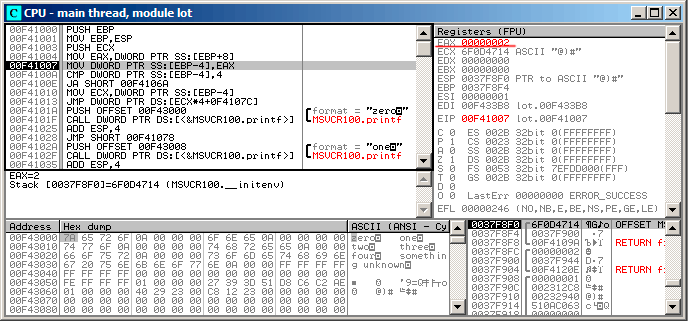
\includegraphics[scale=\FigScale]{patterns/08_switch/2_lot/lot_olly1.png}
\caption{\olly: \RU{входное значение ф-ции загружено в}\EN{function's input value is loaded in} \EAX}
\label{fig:switch_lot_olly1}
\end{figure}

\clearpage
\RU{Входное значение проверяется, не больше ли оно чем}\EN{Input value is checked, if it's bigger than} $4$? 
\RU{Нет, переход по умолчанию (``default'') не будет исполнен}\EN{No, ``default'' jump is not 
taken}:
\begin{figure}[H]
\centering
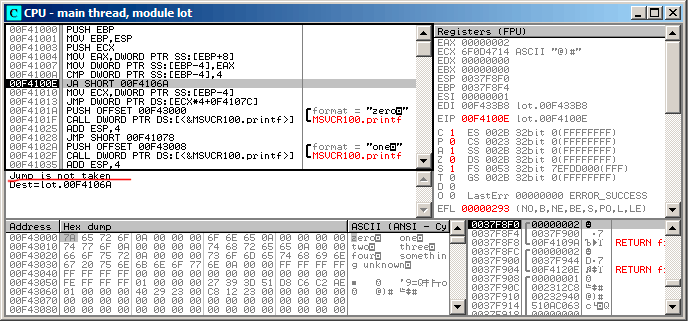
\includegraphics[scale=\FigScale]{patterns/08_switch/2_lot/lot_olly2.png}
\caption{\olly: $2$ \RU{не больше чем}\EN{is no bigger than} $4$: \RU{переход не сработает}\EN{no jump is taken}}
\label{fig:switch_lot_olly2}
\end{figure}

\clearpage
\RU{Здесь мы видим}\EN{Here we see a} jumptable:

\begin{figure}[H]
\centering
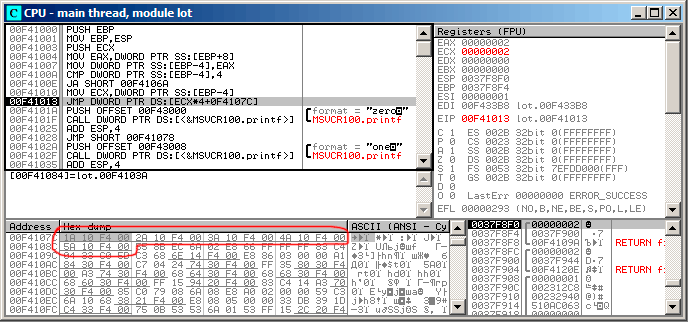
\includegraphics[scale=\FigScale]{patterns/08_switch/2_lot/lot_olly3.png}
\caption{\olly: \RU{вычисляем адрес для перехода используя}\EN{calculating destination address using} jumptable}
\label{fig:switch_lot_olly3}
\end{figure}

\RU{Кстати, я кликнул}\EN{By the way, I clicked} ``Follow in Dump'' $\rightarrow$ ``Address constant'', 
\RU{так что теперь jumptable видна в окне данных}\EN{so now we see a jumptable in data window}. 
\RU{Это 5 32-битных значения}\EN{These are 5 32-bit values}\footnote{\EN{They are underlined by \olly because
these are also FIXUPs}\RU{Они подчеркнуты в \olly, потому что это также и FIXUP-ы}: \ref{subsec:relocs}, 
\RU{мы вернемся к ним позже}\EN{we will back to them later}}.
\ECX \RU{содержит сейчас}\EN{is} $2$\RU{, так что второй элемент (считая с нулевого) таблицы сейчас
будет использован}\EN{ now, so the second element (counting from zeroth) of table will be used}.
\RU{Кстати, можно также кликнуть}\EN{By the way, it's also possible to click} ``Follow in Dump'' $\rightarrow$ 
``Memory address'' \AndENRU \olly \RU{покажет элемент, который сейчас адресуется в инструкции \JMP}\EN{will
show the element \JMP instruction being address now}. 
\RU{Это}\EN{That's} \TT{0x00F4103A}.

\clearpage
\RU{Переход сработал и мы теперь на}\EN{Jump occured and we now at} \TT{0x00F4103A}: 
\RU{сейчас будет исполнен код выводящий строку}\EN{the code printing} ``two''\EN{ string will now be executed}:

\begin{figure}[H]
\centering
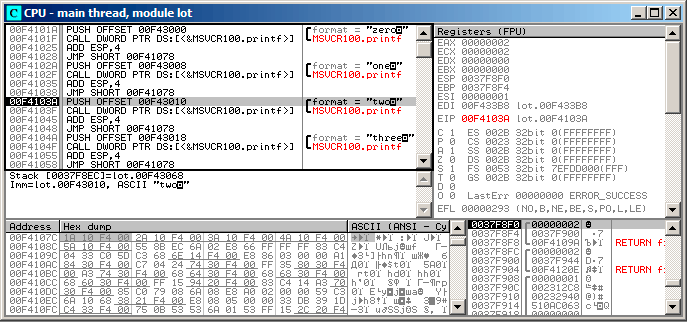
\includegraphics[scale=\FigScale]{patterns/08_switch/2_lot/lot_olly4.png}
\caption{\olly: \RU{теперь мы на соответствующей метке}\EN{now we at corresponding} \IT{case:}\EN{ label}}
\label{fig:switch_lot_olly4}
\end{figure}
\fi

\subsubsection{\NonOptimizing GCC}
\label{switch_lot_GCC}

\RU{Посмотрим, что сгенерирует GCC 4.4.1}\EN{Let's see what GCC 4.4.1 generates}:

\lstinputlisting[caption=GCC 4.4.1]{patterns/08_switch/2_lot/lot_gcc.asm}

\index{x86!\Registers!JMP}
\RU{Практически то же самое, за исключением мелкого нюанса: аргумент из \TT{arg\_0} умножается на 4 
при помощи сдвига влево на 2 бита (это почти то же самое что и умножение на 4)~(\ref{SHR}).
Затем адрес метки внутри функции берется из массива \TT{off\_804855C} и адресуется при помощи 
вычисленного индекса.}
\EN{It is almost the same, except little nuance: argument \TT{arg\_0} is multiplied by 4 by
shifting it to left by 2 bits (it is almost the same as multiplication by 4)~(\ref{SHR}).
Then label address is taken from \TT{off\_804855C} array, address is calculated and stored into 
\EAX, then \TT{``JMP EAX''} do actual jump.}

